\documentclass{beamer}
\usetheme{metropolis}
\usepackage{latexsym}
\usepackage{amssymb}
\usepackage{amsbsy}
\usepackage{alltt}
\usepackage{tikz}
\usetikzlibrary{shapes}
\usepackage{stmaryrd}
\usepackage{graphicx}

\newcommand{\imp}{\Rightarrow}
\newcommand{\etal}{\textit{et. al}}
\newcommand{\adhoc}{\textit{ad hoc}}
\newcommand{\ie}{\textit{i.e.}}
\newcommand{\etc}{\textit{etc}}
\newcommand{\eg}{\textit{e.g.}}
\newcommand{\kemph}[1]{\colorbox{orange}{#1}}
\newcommand{\konst}[1]{\ensuremath{\mbox{\bf{#1}}}}
\newcommand{\nil}{\konst{[\,]}}
\newcommand{\cons}[2]{{#1}\boldsymbol{:}\boldsymbol{:}{#2}}
\newcommand{\hollamb}{\boldsymbol{\lambda}}
\newcommand{\itelse}[3]{\mbox{$\mbox{\tt if}\ {#1}\ \mbox{\tt then}\ {#2}\
    \mbox{\tt else}\ {#3}$}}
\newcommand{\set}[1]{\{ {#1} \}}
\newcommand{\Lang}[1]{\ensuremath{{\cal L}({#1})}}
\newcommand{\LangTheta}[1]{\ensuremath{{\mathcal L}_{\theta}({#1})}}
\newcommand{\inbox}[1] {\begin{center}
                         \framebox{\parbox{0.984\textwidth}{#1}}
                         \end{center}}

% for backslashes in alltt environments
\newcommand{\bs}{\texttt{\symbol{92}}}

\begin{document}

% Title page

\author{Konrad Slind \\ Collins Aerospace}
\date{SafeDocs PI Meeting \par Nov. 10, 2020}
\title{Specifying Message Formats \\ with Contiguity Types}
\maketitle

\begin{frame}\frametitle{Overview}

\begin{enumerate}
\item Context: Architectural Transformations in \konst{CASE}
\item Self-Describing Messages
\item Contiguity Types
\item Extensions and Future Work
\end{enumerate}
\end{frame}


\section {Context: Architectural Transformations in CASE}

\begin{frame}\frametitle{System Architecture Languages}
\begin{itemize}

\item General setting: \textbf{Architectural Design Languages}

\item An ADL supports complete, highly abstract, views of a system,
  including hardware, software, (and possibly humans)

\item An architecture model should provide a high-level setting in which
  the \kemph{whole picture} of a system can be surveyed

\item Thus: a place where existing implementations, new design
  features, high-level requirements, implementations, and
  verifications can be combined.

\item Not just boxes and arrows!

\end{itemize}

\end{frame}

\begin{frame}\frametitle{CASE}
\begin{itemize}

\item In the DARPA \textbf{CASE} project we are developing the idea of
  \kemph{Security-Enhancing} transformations on system architecture
  descriptions.

\item Acronym: \colorbox{orange}{SEAT}

\item The goal is to develop a methodology and case studies where
  \begin{itemize}
  \item [$\blacktriangleright$]
       the structure of an existing (legacy) system is captured in an architectural model;

 \item [$\blacktriangleright$] system security is automatically analyzed and any security
   problems are addressed by applying architectural transformations
 \end{itemize}

\item A key aspect is use of formal specification languages and
  automatic synthesis of security mechanisms.

\end{itemize}

\end{frame}

\begin{frame}[fragile]\frametitle{CASE Website}

Check it out:

\begin{verbatim}
  http://loonwerks.com/projects/case.html
\end{verbatim}

\end{frame}


\begin{frame}\frametitle{Architecture Transformations}

An architecture-to-architecture map that can be applied to
\kemph{provably increase} the security of a system.

\vspace*{4mm}

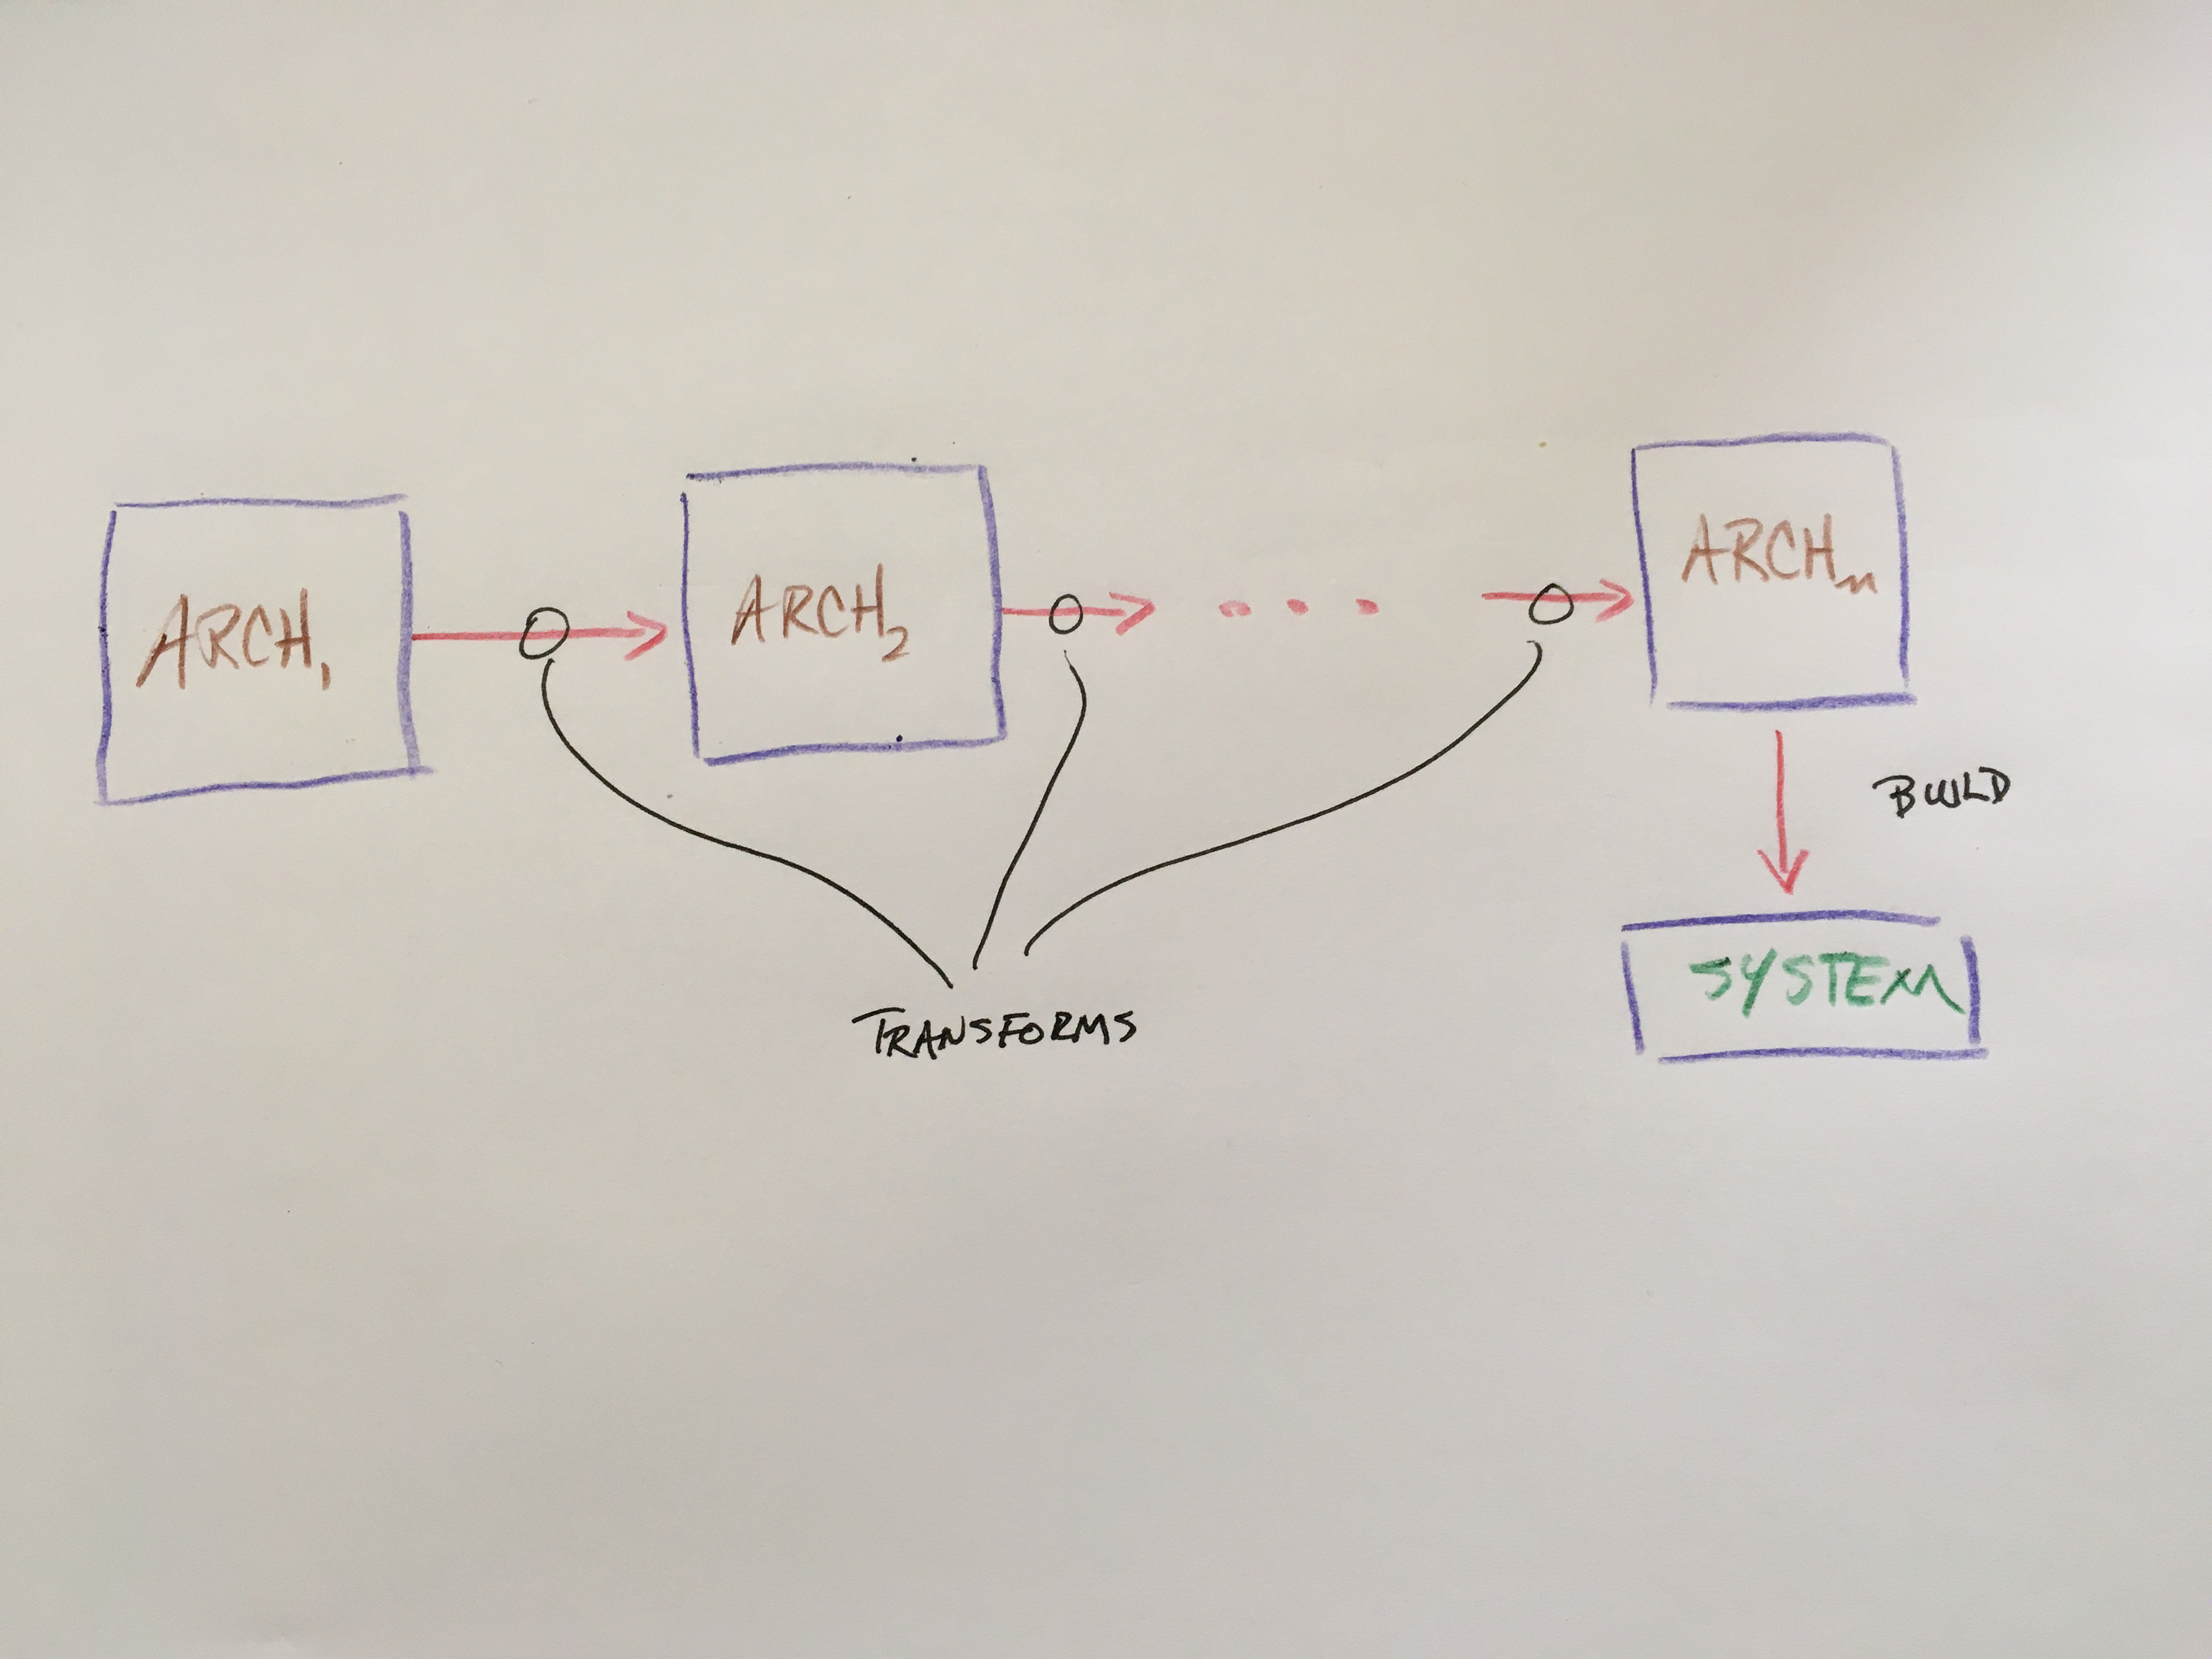
\includegraphics[width=90mm,height=50mm]{arch-trans.jpg}
\end{frame}

\begin{frame}\frametitle{Transformation: Message Filtering}

A \emph{filter} is conceptually very simple: it checks validity of its
input data according to predicate $P$.


\begin{center}
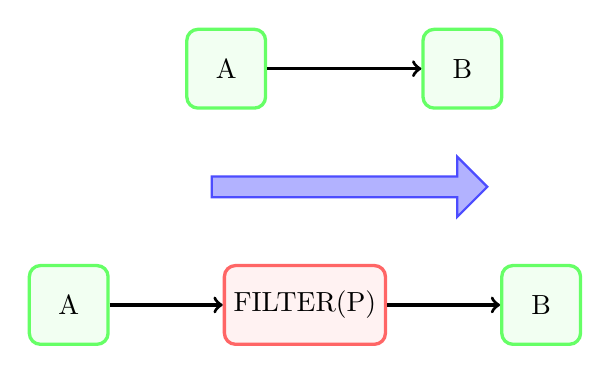
\begin{tikzpicture}[
redsquarednode/.style={rectangle, draw=red!60, fill=red!5, very thick, rounded corners, minimum size=10mm},
greensquarednode/.style={rectangle, draw=green!60, fill=green!5, very thick, rounded corners, minimum size=10mm},
fat arrow/.style={single arrow,thick,draw=blue!70,fill=blue!30,minimum height=35mm,minimum width=7mm}
]
%Nodes
\node[draw,greensquarednode] at (2,0) (SRC)    {A};
\node[draw,greensquarednode] at (5,0) (TARGET) {B};

\node at (3.5,-1.5) [fat arrow]{};

\node[draw,greensquarednode] at (0,-3) (SRC-1)    {A};
\node[draw,greensquarednode] at (6,-3) (TARGET-1) {B};
\node[draw,redsquarednode] at (3,-3) (FILTER) {FILTER(P)};

%Lines
\draw[->,very thick] (SRC.east) -- (TARGET.west);

\draw[->,very thick] (SRC-1.east) -- (FILTER.west);
\draw[->,very thick] (FILTER.east) -- (TARGET-1.west);
\end{tikzpicture}
\end{center}

%% \hspace*{10mm}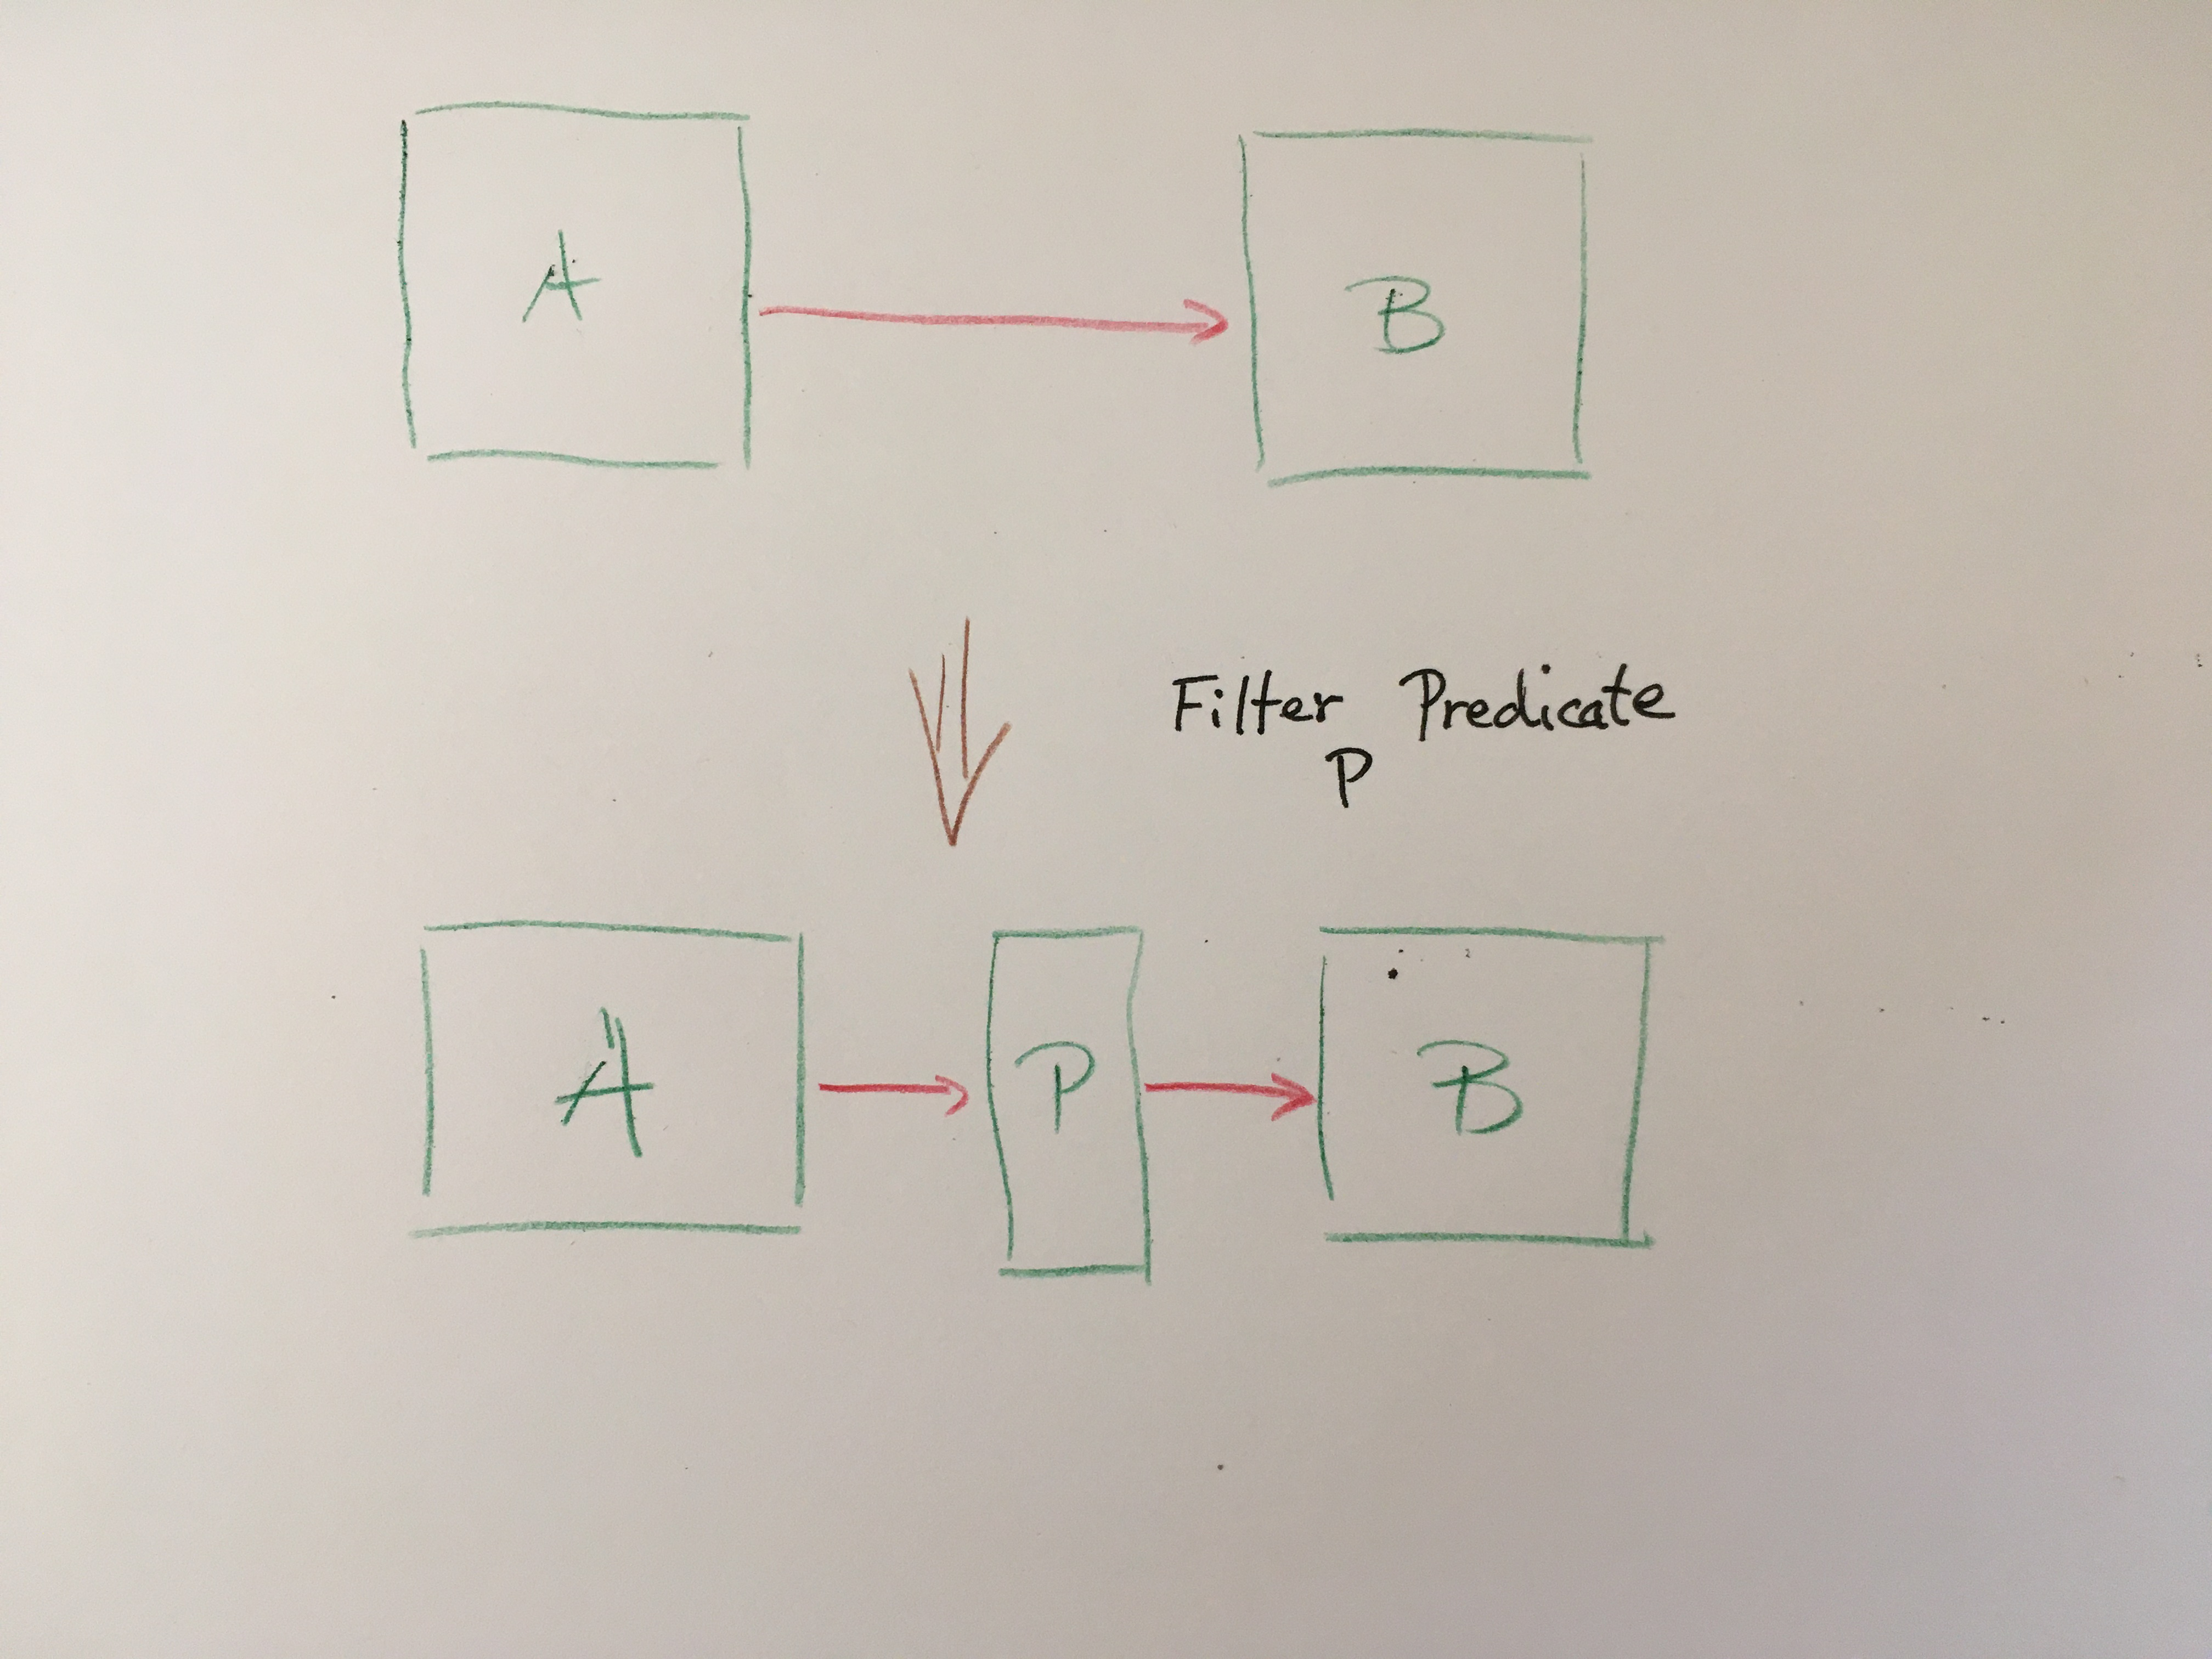
\includegraphics[width=90mm,height=50mm]{filter.jpg}

If the data is valid, then it is passed on. Otherwise it is dropped.

\end{frame}


\begin{frame}\frametitle{Transformation: Message Monitoring}

A \emph{monitor} checks to see that a relationship $\mathcal{R}$ holds
over a collection of message streams through time. If the
specification is violated, an \emph{alert} is sent out.

\begin{center}
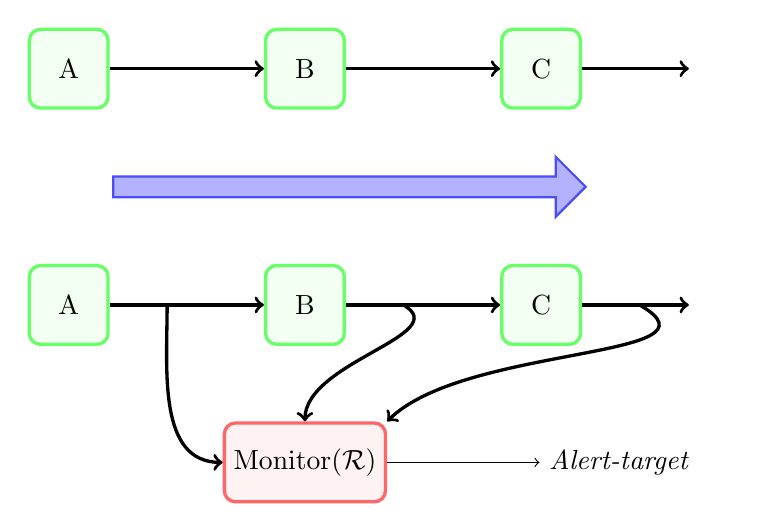
\begin{tikzpicture}[
redsquarednode/.style={rectangle, draw=red!60, fill=red!5, very thick, rounded corners, minimum size=10mm},
greensquarednode/.style={rectangle, draw=green!60, fill=green!5, very thick, rounded corners, minimum size=10mm},
fat arrow/.style={single arrow,thick,draw=blue!70,fill=blue!30,minimum height=60mm,minimum width=7mm}
]
%Nodes
\node[draw,greensquarednode] at (1,0) (A) {A};
\node[draw,greensquarednode] at (4,0) (B) {B};
\node[draw,greensquarednode] at (7,0) (C) {C};
\node at (9,0) (D) {};

\node at (4.5,-1.5) [fat arrow]{};

\node[draw,greensquarednode] at (1,-3) (A-1) {A};
\node at (2.25,-3) (joinAB) {};
\node[draw,greensquarednode] at (4,-3) (B-1) {B};
\node at (5.25,-3) (joinBC) {};
\node[draw,greensquarednode] at (7,-3) (C-1) {C};
\node at (8.25,-3) (joinCD) {};
\node at (9,-3) (D-1) {};
\node[draw,redsquarednode]   at (4,-5) (M) {Monitor($\mathcal{R}$)};
\node at (8,-5) (ALERT-TARGET) {\textit{Alert-target}};

%Lines
\draw[->,very thick] (A.east) -- (B.west);
\draw[->,very thick] (B.east) -- (C.west);
\draw[->,very thick] (C.east) -- (D.west);
\draw[->,very thick] (A-1.east) -- (B-1.west);
\draw[->,very thick] (B-1.east) -- (C-1.west);
\draw[->,very thick] (C-1.east) -- (D-1.west);

\draw[->,very thick] (2.25,-3) to [out=-90, in=180] (M);
\draw[->,very thick] (5.25,-3) to [out=-30, in=90]  (M);
\draw[->,very thick] (8.25,-3) to [out=-30, in=45]  (M.north east);
\draw[->] (M.east) -- (ALERT-TARGET);

\end{tikzpicture}
\end{center}

%% \hspace*{10mm}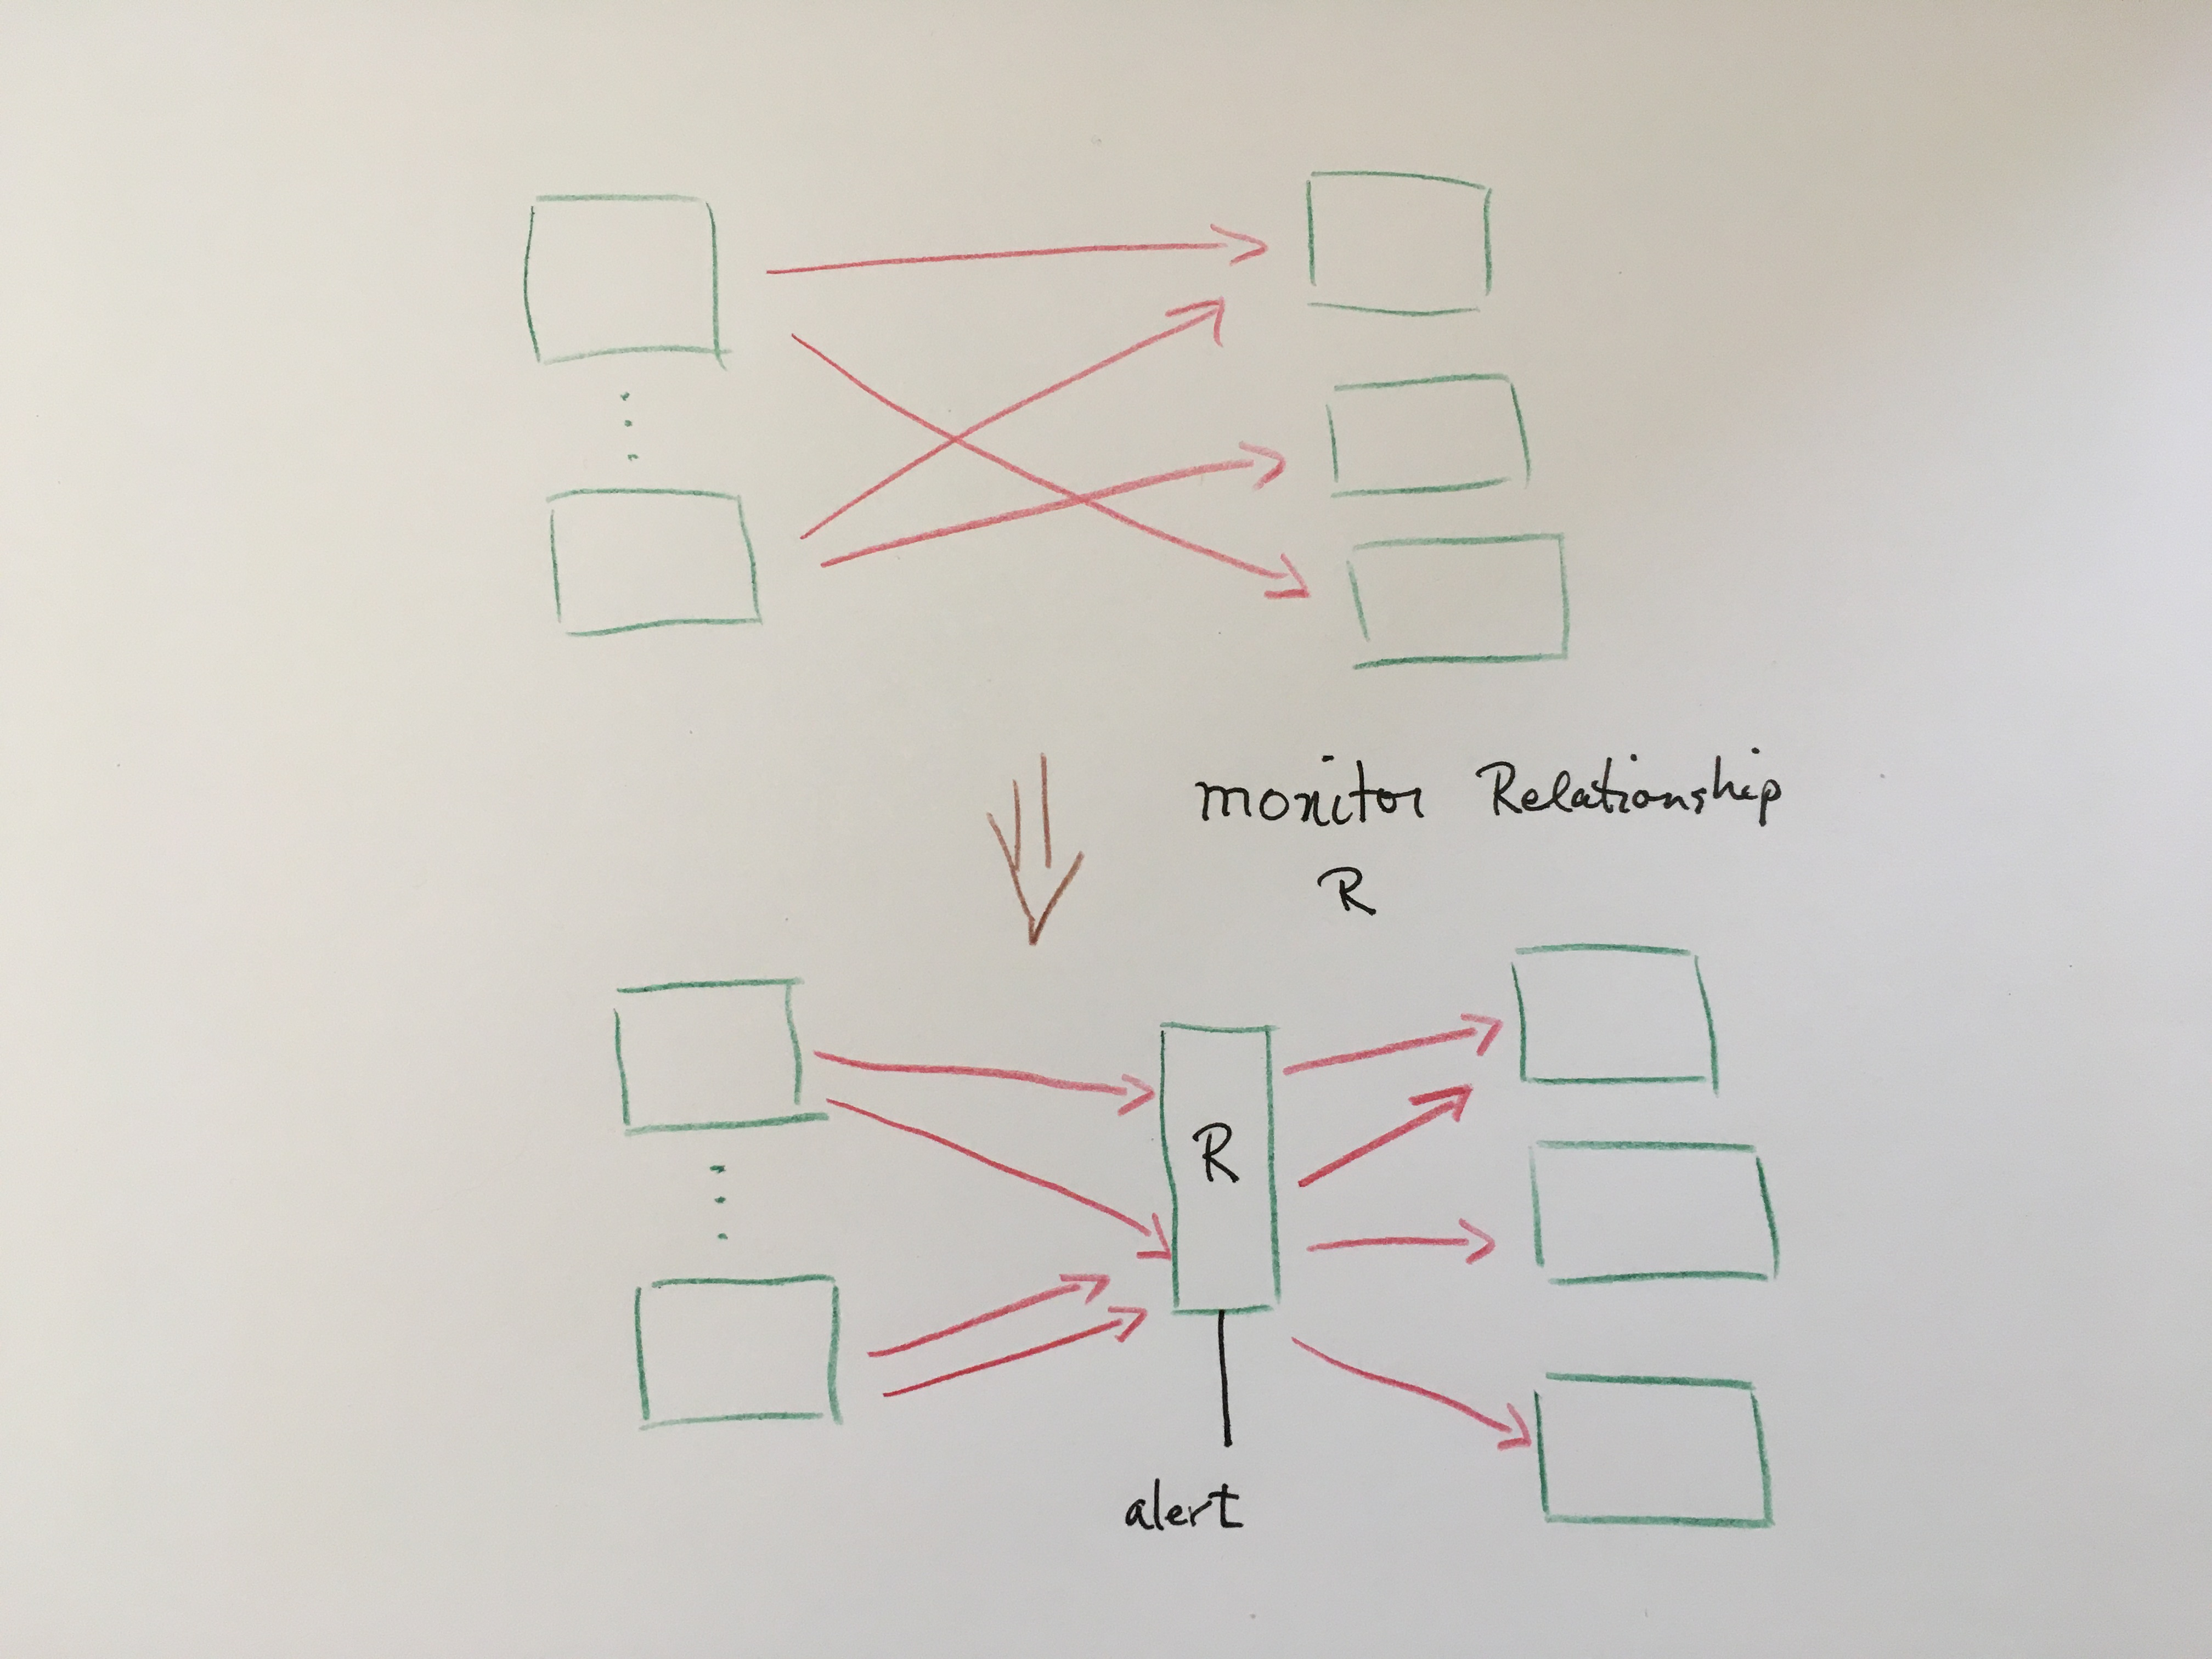
\includegraphics[width=90mm,height=40mm]{monitor.jpg}

\end{frame}

\begin{frame}\frametitle{Transformation: Message Monitoring}

  We currently use past-time temporal logic to specify monitors, following

\begin{quote}\
Efficient Monitoring of Safety Properties, Havelund and Rosu, TACAS 2002.
\end{quote}

\end{frame}


\begin{frame}\frametitle{Transformation: Isolation of `at risk' components}

An unprotected computational element can be isolated by transparently
lifting it out of its context and mediating access via seL4.

\begin{center}
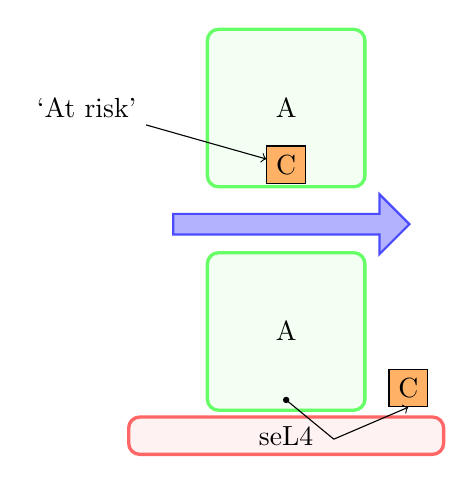
\begin{tikzpicture}[
bignode/.style =
  {rectangle,
   draw=green!60, fill=green!5,
   very thick, rounded corners,
   minimum height=20mm, minimum width = 20mm},
flatnode/.style =
  {rectangle,
   draw=red!60, fill=red!5,
   very thick, rounded corners,
   minimum width = 40mm},
fat arrow/.style={single arrow,thick,draw=blue!70,fill=blue!30,minimum height=30mm,minimum width=7mm}
]
%Nodes
\node[draw,bignode](main){A};
\node[draw,fill=orange!60] (atrisk) at ([yshift=2ex]main.south){C};
\node (comment) at ([xshift=-10ex]main.west){`At risk'};
\draw[->] (comment) -- (atrisk);
\node at ([yshift=-3ex]main.south) [fat arrow]{};
\node[draw,bignode](main-1) at ([yshift=-12ex]main.south){A};
\node[draw,fill=orange!60] (secure) at ([xshift=3.5ex,yshift=2ex]main-1.south east){C};
\node[draw,flatnode] (seL4) at ([yshift=-2ex]main-1.south){seL4};
\node[draw,fill=black,circle,scale = 0.2] (origin) at ([yshift=1ex]main-1.south){};
\node (foo) at ([yshift=-2ex,xshift=4ex]seL4.north){};
\draw (origin) -- (foo.center);
\draw[->] (foo.center) -- (secure.south);
\end{tikzpicture}
\end{center}

%\filldraw[black] (0,0) circle (2pt) node[anchor=west] {Intersection point};
%\hspace*{10mm}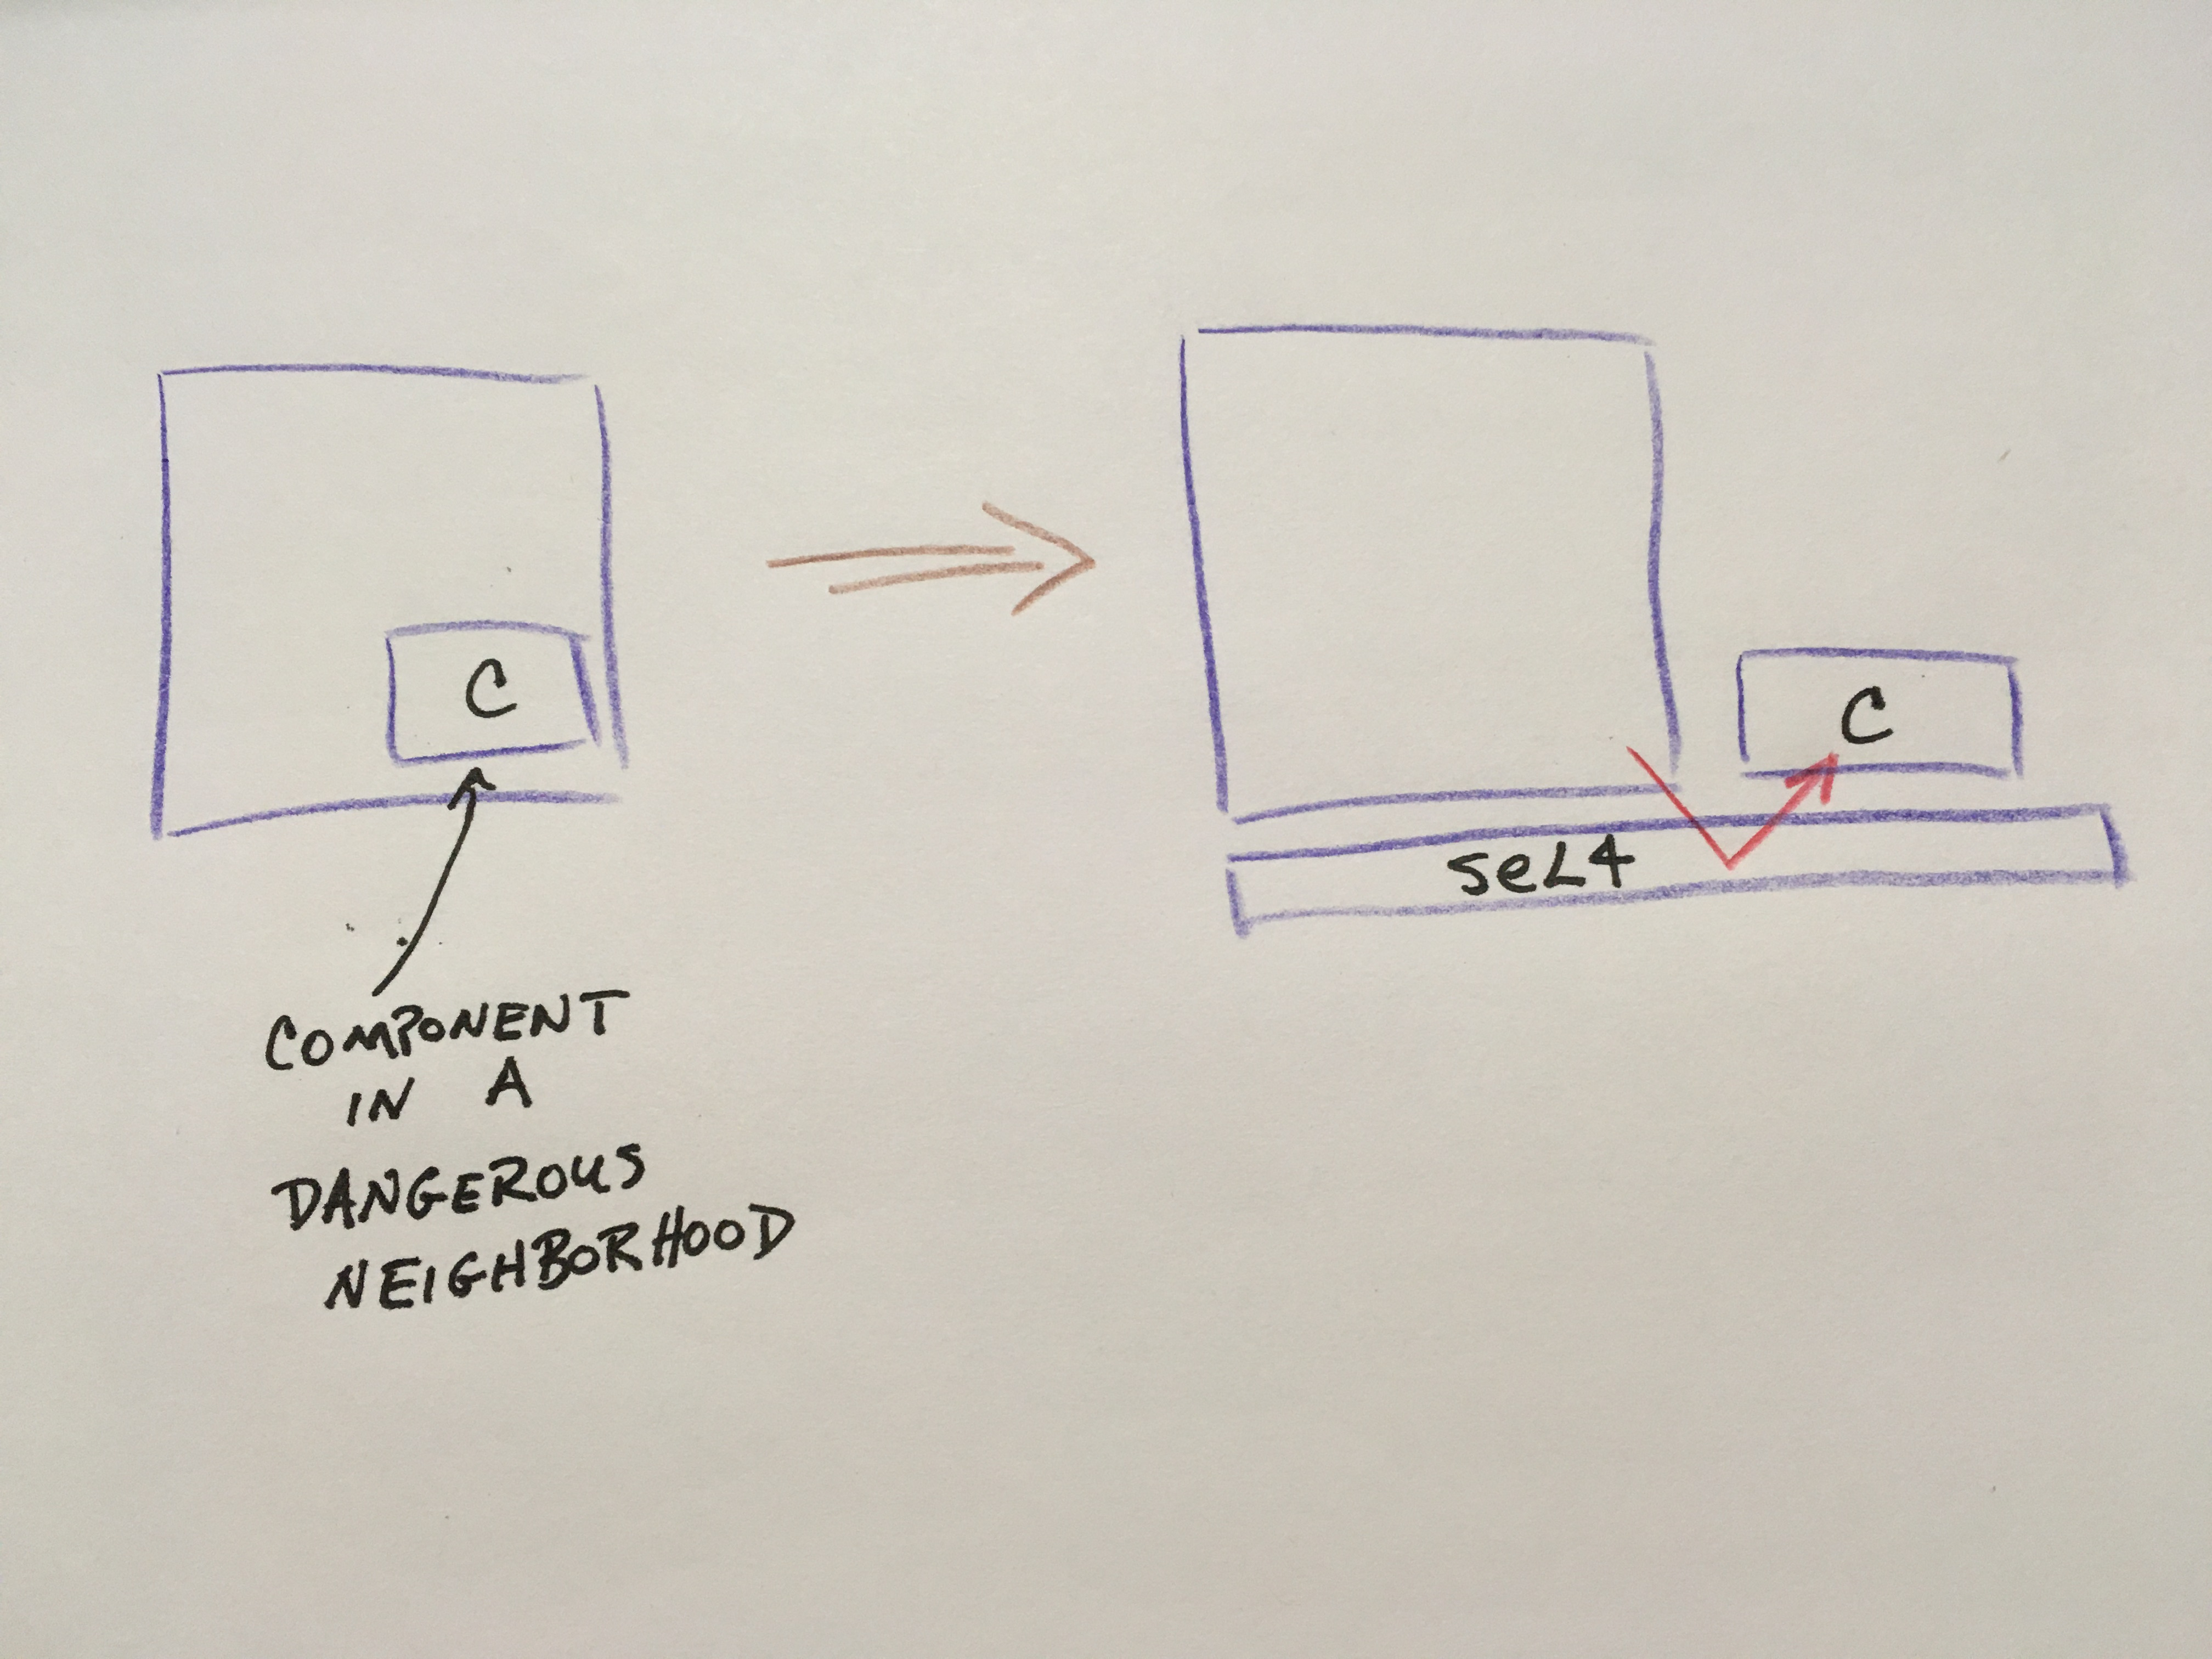
\includegraphics[width=90mm,height=40mm]{vm.jpg}

\end{frame}

\begin{frame}\frametitle{seL4}

Correctness of this transformation depends on formal guarantees provided by seL4.

\begin{itemize}
\item seL4 microkernel guarantees partitioning of components and
  communication, backed by computer-checked proofs

\item seL4 guarantees no infiltration, exfiltration, eavesdropping,
  interference, and provides fault containment for untrusted code

\end{itemize}

\vspace*{5mm}
\hspace*{10mm}
\includegraphics[width=15mm,height=15mm]{data61-logo.png}
\hspace*{10mm}
\includegraphics[width=15mm,height=15mm]{csiro--black.png}

\end{frame}

\begin{frame}\frametitle{Transformation: Attestation}

Attestation inserts measurement mechanisms into a system. These
examine various aspects of system behavior, and send summaries back to
an observer system.

%% %% \newcommand\rightEye[1][1.2ex]
%% %% {%
%% %% \begin{tikzpicture}[scale=#1/1cm]
%% %%   \draw (0,0) circle (.5);
%% %%   \fill (.25,0) circle (.25);
%% %% \end{tikzpicture}%
%% %% }

%% \begin{center}
%% \begin{tikzpicture}[
%% lefteyes/.style =
%%   {circle,
%%    draw=red!60, fill=red!5,
%%    minimum height=20mm, minimum width = 20mm}
%% ]
%% %Nodes
%% \draw (0,0) rectangle (1,1);
%% \draw (3,0) rectangle (1,1);

%% \draw (0,-3) rectangle (1,1);
%% \draw (3,-3) rectangle (1,1);
%% \draw (3,-3.5) rectangle (0.5,0.5);

%% \draw (3,-4) circle (.5);
%% \fill (3.25,-4) circle (.25);
%% \end{tikzpicture}
%% \end{center}

\hspace*{10mm}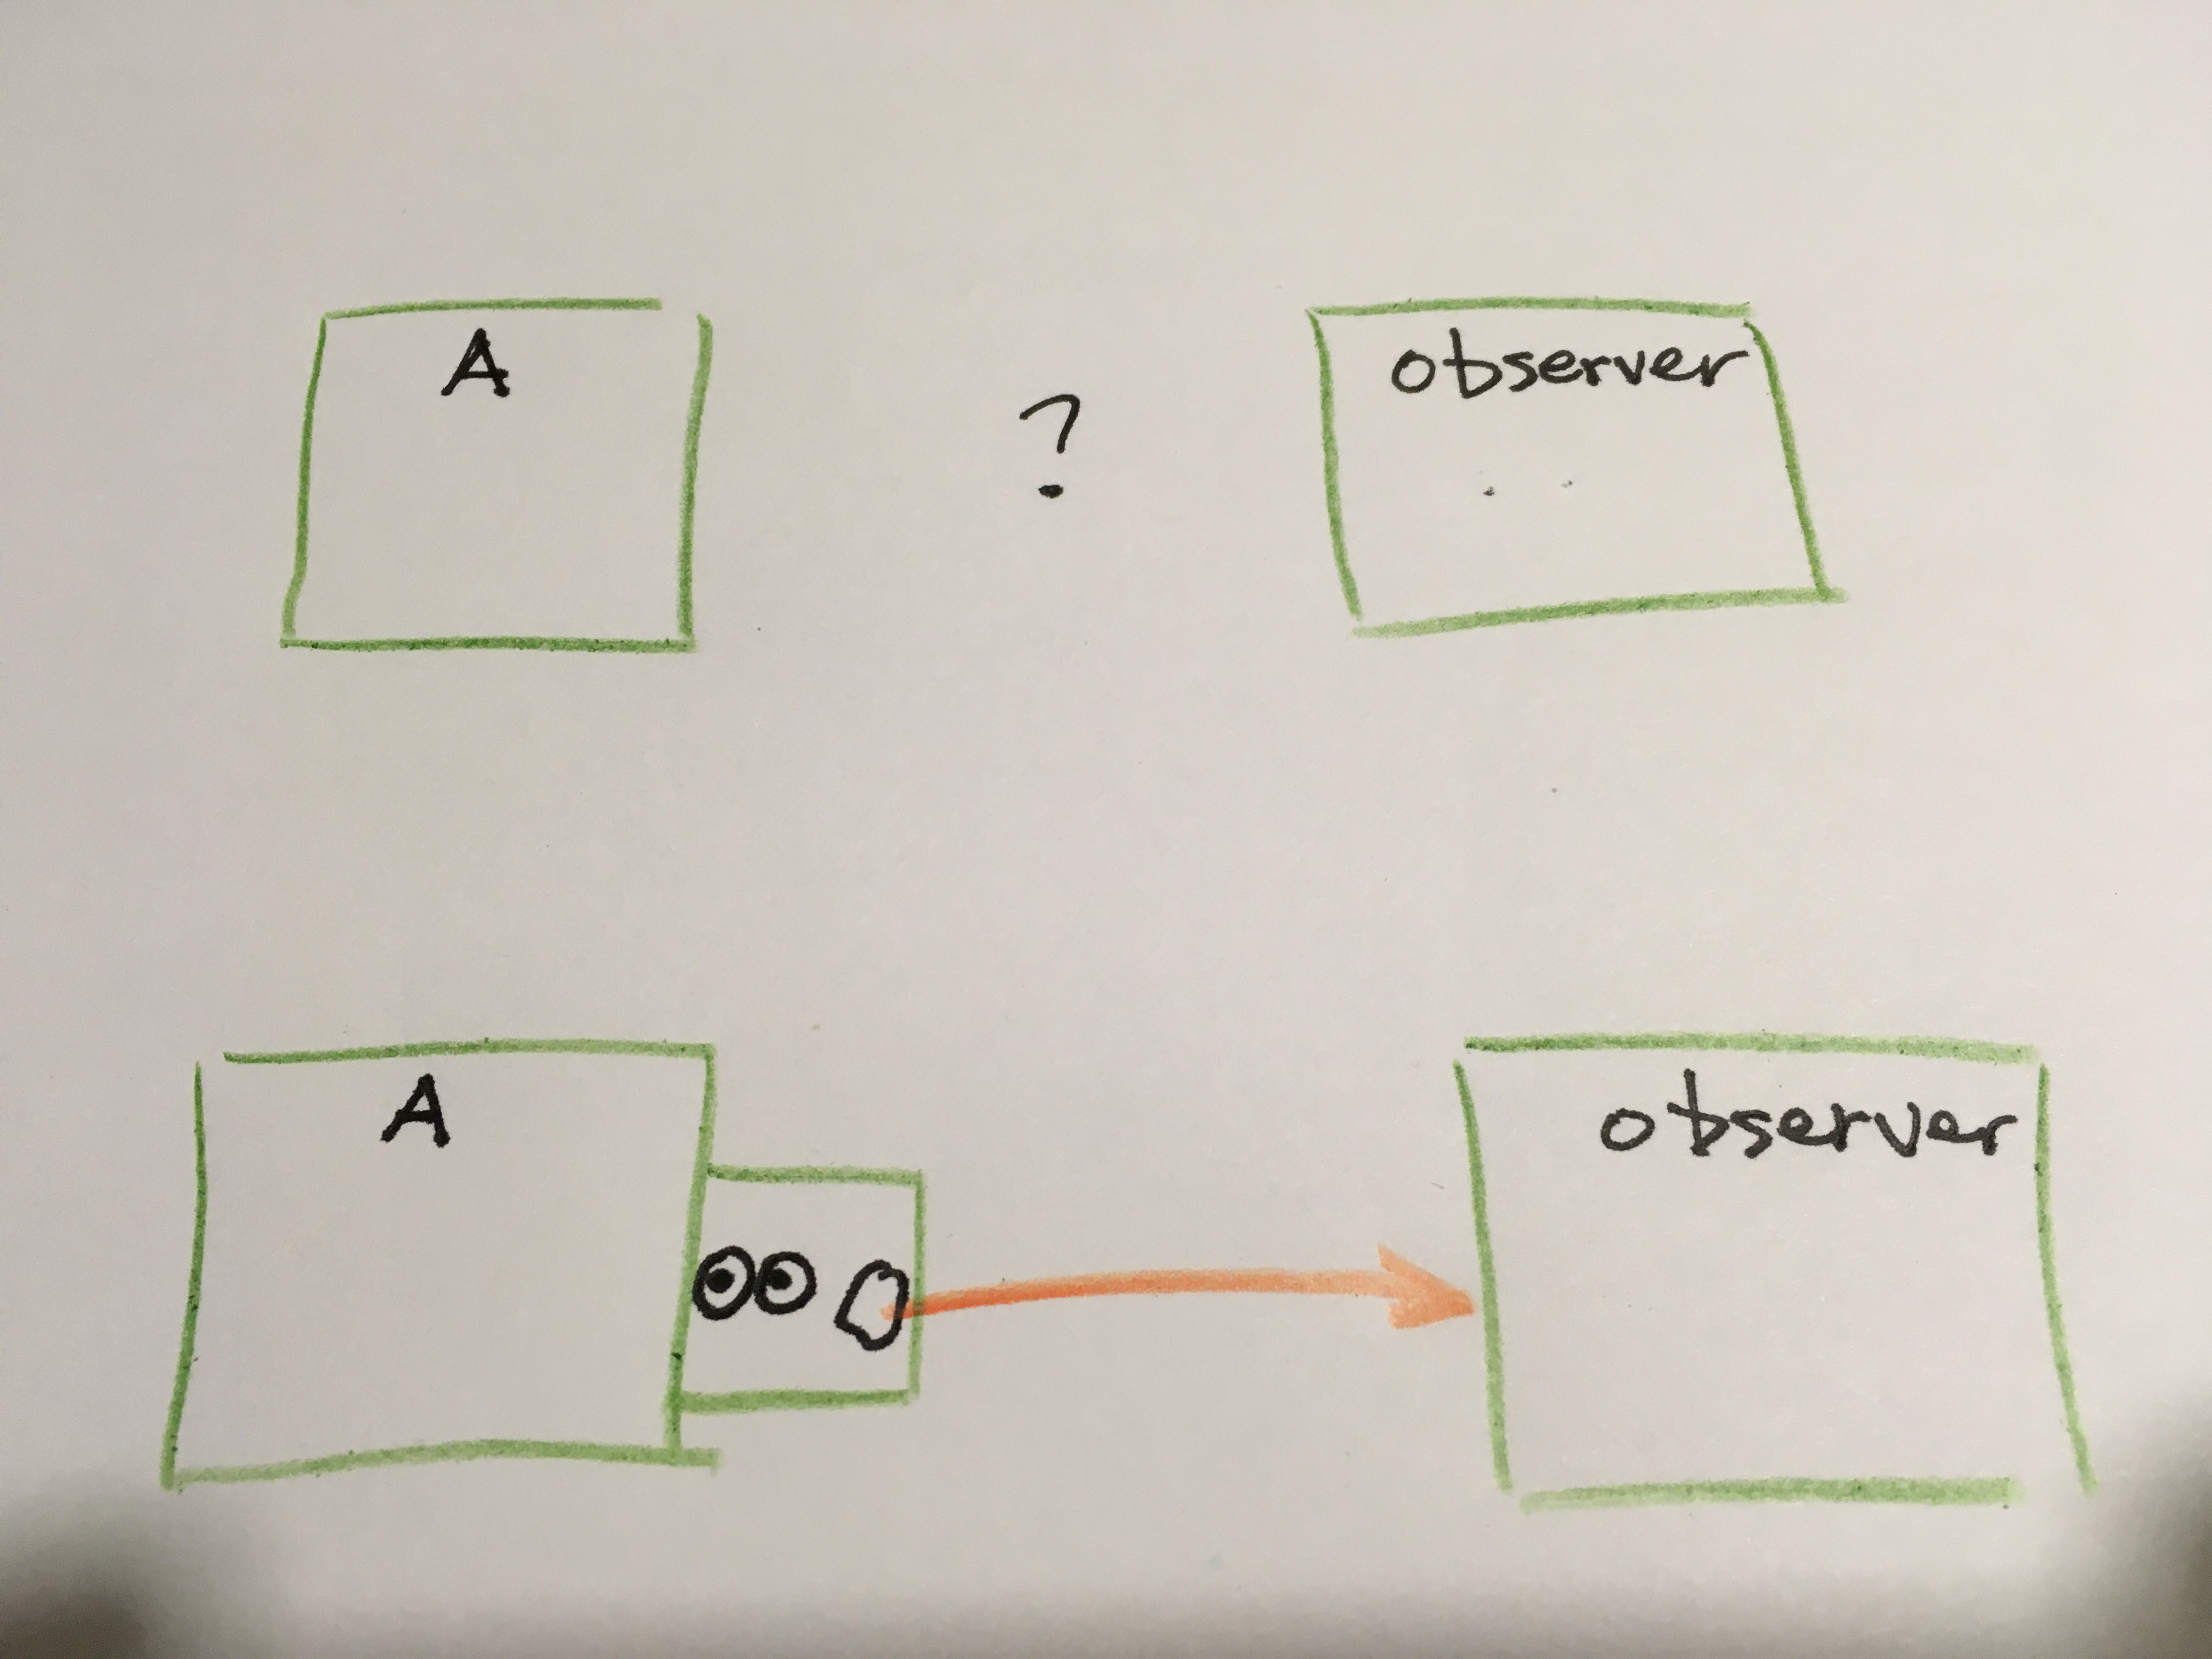
\includegraphics[width=90mm,height=40mm]{att.jpg}


\end{frame}

\begin{frame}\frametitle{CakeML implementations}

  The filter, monitor, and attestation transforms generate \konst{CakeML} implementations.

\begin{itemize}
 \item [$\blacktriangleright$] CakeML is a formally verified ML compiler

\item This allows a theorem that connects the high-level spec of a
  component with the execution of the binary on an ISA.
\end{itemize}

\end{frame}


\section {Specifying Message Formats}

\begin{frame}\frametitle{Ports vs messages}

Question: what does a filter operate over?

\begin{itemize}

\item In AADL a component communicates with other components via
  \kemph{typed connections}

\item Port types are the usual finite types from programming:
  booleans, integers, floats, arrays, records, unions, etc.

\item Properties in our specification language are therefore
  written over these port types.

\item In particular, the `add-a-filter' transform is specified by a predicate over the input port type.

\end{itemize}

\end{frame}

\begin{frame}[fragile]\frametitle{Example : Wellformed GPS coordinates}

{\small
\begin{verbatim}
 AltitudeType = AGL | MSL

 Location3D = {
  Latitude  : real64,
  Longitude : real64,
  Altitude  : real32,
  AltitudeType : AltitudeType}

 Good_Location (loc) =
    -90.0 <= loc.Latitude <= 90.0 and
   -180.0 <= loc.Longitude <= 180.0 and
      0.0 <= loc.Altitude <= 15000.0
\end{verbatim}
}

\end{frame}

\begin{frame}\frametitle{Example : Wellformed GPS strings}

However, in the implementation, messages coming into a port are byte
arrays (essentially untyped).

\[
\begin{array}{l}
 \konst{Good\_Location\_Mesg} (s) \iff \\
\quad   \exists s_1 s_2 s_3 s_4. \\
\qquad      s = s_1 \bullet s_2 \bullet s_3 \bullet s_4 \ \land \\
\qquad    -90.0 \leq \konst{doubleVal}(s_1) \leq 90.0 \ \land \\
\qquad   -180.0 \leq \konst{doubleVal}(s_2) \leq 180.0 \ \land \\
\qquad      0.0 \leq \konst{floatVal}(s_3)  \leq 15000.0 \ \land \\
\qquad        0 \leq \konst{natVal}(s_4) \leq 1
\end{array}
\]
%
\noindent where
%
\[
\begin{array}{ll}
 \konst{doubleVal} & : \konst{string} \to \konst{double} \\
 \konst{floatVal}  & : \konst{string} \to \konst{float}  \\
 \konst{natVal}    & : \konst{string} \to \konst{nat}  \\
\end{array}
\]

\end{frame}

\begin{frame}\frametitle{SPLAT}

We need to span the gap between specifications on high level data and
implementations over flat strings.

Seek to apply ideas from Formal Language Theory to showing properties
of operations on high-level data.

\vspace*{10mm}

\kemph{\konst{SPLAT} = Semantic Properties over Language and Automata Theory}

\end{frame}

\begin{frame}[fragile]\frametitle{SPLAT the early days}

Initial version of \konst{SPLAT} was based on a HOL4 theory of regexps and regexp
compilation developed with Scott Owens.

\begin{itemize}[<+->]
\item [$\blacktriangleright$] Regard a message as a concatenation of \emph{fields}
\item [$\blacktriangleright$] Each field has an interval spec of the form $\mathit{lo} \leq \mathit{field} \leq \mathit{hi}$
\item [$\blacktriangleright$] An interval spec can be translated to a regexp which is a
  predicate on the binary representation of the field.
\item The concatenation of regexps for the message fields gives a big regexp for the message.
\item [$\blacktriangleright$] Filter is obtained by compiling (deductively) regexp to DFA.
\end{itemize}

\end{frame}

\section{Self-describing messages}

\begin{frame}[fragile]\frametitle{Self-describing messages}

Unfortunately, many message formats can't be captured by regexps.

Message formats commonly have self-describing aspects such as

\begin{itemize}

\item \kemph{length} fields, which represent sizes for other parts of
  the message, e.g., a list of elements, paired with its length

\item \kemph{unions}, which allow multiple versions of a format to
  exist in a single format, e.g.  \textit{If field A is less than 14
    then the message has 10 fields, else it has 15}

\end{itemize}

In general, \kemph{the deeper you go the more you know} and we need to
do a good job of modelling that accumulation of information while
recognizing/parsing.

\end{frame}

\begin{frame}\frametitle{Approaches to self-describing messages}

\begin{itemize}

\item Many message format description languages have been invented over time.

\item Wouldn't it be great if the vast ocean of formal language theory could be applied?

\item The self-describing aspect, unfortunately, hampers the use of
  standard lexer and parser technology

\item Regular languages are insufficient (as noted) and context-free
  grammars can’t capture the dependency of one field (or collection of
  fields) on another.

\end{itemize}
\end{frame}

\begin{frame}\frametitle{Approaches to self-describing messages}
\begin{itemize}

\item Context-sensitive grammars seem like a possibility, but there is
  very little tool support for them

\item Parser combinators allow  hand-rolled parsers to be very quickly
  constructed, and can be adapted to support the accumulation and
  propagation of the necessary dependency information.

\item Also an impressive body of work using dependent types in Coq

\end{itemize}

However we would like to stay on the formal language side of things
for now since there is a strong connection between messages (sequences
of bits/bytes) and the strings of formal language theory.

\end{frame}

\begin{frame}[fragile]\frametitle{Contiguity types}

  The notion is that message processing consists of

\begin{itemize}
\item accumulating field information
\item computing values from that information when needed
\end{itemize}

In particular, we need

\begin{itemize}
\item \kemph{Arithmetic} expressions for computing length fields
\item \kemph{Boolean} expressions for computing decisions in unions
\end{itemize}

\end{frame}

\begin{frame}[fragile]\frametitle{Contiguity types: syntax}

The syntax of contiguity types is very similar to a standard
collection of base types closed under formation of records and arrays.

\[
\begin{array}{rcl}
 \mathit{base} & = & \konst{bool} \mid \konst{char} \mid \konst{u8} \mid
 \konst{u16} \mid \konst{u32} \mid \konst{u64}  \mid \konst{i16} \mid
 \konst{i32} \mid \konst{i64} \mid \konst{f32} \mid \konst{f64} \\
 \tau & = & \mathit{base} \\
      & \mid & \konst{Recd}\; (f_1 : \tau_1) \ldots (f_n : \tau_n) \\
      & \mid & \konst{Array}\; \tau \; \mathit{exp} \\
      & \mid & \konst{Union}\; (\mathit{bexp}_1 : \tau_1) \ldots (\mathit{bexp}_n : \tau_n)
\end{array}
\]
\end{frame}

\begin{frame}[fragile]\frametitle{Contiguity types: examples}

%% \fbox{
%% \begin{verbatim}
%%   {A : char
%%   B  : i32
%%   C  : u32 [1024]}
%% \end{verbatim}
%% }

\begin{tabular}{ll}
Simple record &
\fbox{
\begin{tabular}{rcl}
  \{A & : & char \\
  B & : & i32 \\
  C & : & u32 [1024]\}
\end{tabular}
}
\\ \\

Array &
\fbox{
\begin{tabular}{rcl}
  \{len & : & u16 \\
   A   & : & i32 [\kemph{len}]\}
\end{tabular}
}
\\ \\

Array &
\fbox{
\begin{tabular}{rcl}
  \{Dims & : & \{rows :  u16 \\
         & &   {~} cols : u16\} \\
 Image & : & i32 [\kemph{Dims.rows * Dims.cols}]\}
\end{tabular}
}
\end{tabular}

\end{frame}

\begin{frame}[fragile]\frametitle{Contiguity types: examples}

Union

\fbox{
\begin{tabular}{lcl}
  \{relno & : & u32 \\
  \phantom{\{} B & : & i32 \\
\phantom{\{} C & : & Union (\kemph{relno \textless 14}, \{D : u32 [B]\}) \\
  & & {~~} (\kemph{not(relno \textless 14)}, \{ P : bool, Q : i64 [B]\}\}
\end{tabular}
}

\end{frame}

\begin{frame}[fragile]\frametitle{Contiguity types: semantics}

The semantics of contiguity types is in terms of formal languages:

\[
% \begin{array}{l}
\LangTheta{\tau} =
\mathtt{case}\; \tau\
% \hspace*{3mm}
 \left\{
 \begin{array}{l}
 \mathit{base} \Rightarrow \set{s \mid \konst{len}(s) = \konst{width}(base)} \\
 \konst{Recd}\; (f_1 : \tau_1) \ldots (f_n : \tau_n)
      \Rightarrow \LangTheta{\tau_1} \cdot \ldots \cdot \LangTheta{\tau_n}
\\
 \konst{Array}\; \tau_1 \; \mathit{exp}
      \Rightarrow  \LangTheta{\tau_1}^{\konst{evalExp}\;\theta\;\mathit{exp}}
\\
 \konst{Union}\; (\mathit{bexp}_1 : \tau_1) \ldots (\mathit{bexp}_n : \tau_n) \Rightarrow \\
  \hspace*{5mm}
 \left\{
 \begin{array}{ll}
    \LangTheta{\tau_i} &  \mathrm{if}\ \konst{evalBexp}\;\theta\;\mathit{bexp}_i = \konst{true} \\
                  & \mathrm{and\ no\ other}\ \mathit{bexp}_j\ \mathrm{is}\ \konst{true}  \\
    \emptyset & \mathrm{otherwise}
 \end{array}
 \right.
 \\
\end{array}
 \right.
%\end{array}
\]
\end{frame}

\begin{frame}[fragile]\frametitle{Contiguity types: semantics}

In words:

\begin{itemize}
\item Each base type has a width and the meaning of a base type is the
  set of all strings of the given width.

\item A record translates to the language concatenation of the translations of its fields.

\item An array $\konst{Array}\;\tau\; \mathit{exp}$ is the $n$-ary
  concatenation of the language of $\tau$, where $n$ is the value of
  $\mathit{exp}$.

\item A union $\konst{Union}\; (\mathit{bexp}_1 : \tau_1) \ldots
  (\mathit{bexp}_n : \tau_n)$ maps to the translation of $\tau_i$ if
  $\mathit{bexp}_i$ is the only boolean expression that evaluates to
  \konst{true}.

\end{itemize}

\end{frame}


\begin{frame}\frametitle{Assertions}

Contiguity types can express in-message assertions:

\[
\begin{array}{l}
\konst{Assert}\;\mathit{bexp}  =
\konst{Union}\; (\mathit{bexp}, \konst{SKIP})  (\neg\mathit{bexp}, \konst{VOID}) \\

\konst{SKIP}  =  \konst{Recd} [\, ] \\
\konst{VOID}  =  \konst{Union} (\konst{false}, -)
\end{array}
\]

Declarative reading: evaluate the boolean expression in the current context;
  if it is true then $\varepsilon$ else $\emptyset$,

Operationally: \kemph{check the property; if it's true, continue on; if false, fail.}

\konst{NB} The expressiveness is determined by the type of boolean expressions.

\end{frame}

\begin{frame}[fragile]\frametitle{Assertion example $a^n b^n c^n$}


{\small
\begin{verbatim}
  charA = {ch : char, isA : Assert (ch = 97)}
  charB = {ch : char, isB : Assert (ch = 98)}
  charC = {ch : char, isC : Assert (ch = 99)}

  {A : {len: u16, elts : charA [len]}
   B : {len: u16, elts : charB [len]}
   C : {len: u16, elts : charC [len]}
   check-lang
     : Assert (A.len = B.len and B.len = C.len)
  }
\end{verbatim}
}

\end{frame}

\begin{frame}[fragile]\frametitle{Assertion example: no duplicate keys}

{\small
\begin{verbatim}
  string = {len : u16, elts : char[len]}

  {Dict : {len  : u16,
           elts : {key:string, value: i32} [len]}

   check : Assert (forall i < Dict.len,
                   forall j < Dict.len.
            (Dict.elts[i].key = Dict.elts[j].key iff (i = j)))
  }
\end{verbatim}
}

\konst{NB} The check is happening down at the byte-stream level. No
data structures being built.

\end{frame}

\begin{frame}\frametitle{Matching algorithm}

We have formally defined a function \textbf{match} which takes a
contig type and a string and returns an assignment $\theta$ of slices
of the string to elements of the type.

\begin{theorem}[Soundness]
  \[
 \vdash \konst{match}\; \mathit{contig}\; \mathit{string} = \konst{Some}(\theta) \imp
   \mathit{string} \in \LangTheta{\mathit{contig}}
\]
\end{theorem}

\textbf{match} has the flavor of a \kemph{parser generator}: it takes a
specification of the language to be parsed and returns an implementation

\kemph{We use \textbf{match} to implement all filters in \konst{CASE}.}

\end{frame}


\begin{frame}\frametitle{Matching algorithm}

\begin{itemize}

\item A successful match says that the string meets the constraints of
  the contig type, including all constraints specified via internal
  assertions.


\item Operates in \emph{worklist} style

\item Alternately flattens contig-type down until a base type is exposed

\item At base type, the corresponding chunk of string is consumed and added to context $\theta$

\item There is also an instrumented version which produces parse trees

\item \kemph{Incredibly simple implementation} (approx 200 lines of SML)
\end{itemize}

\end{frame}


\begin{frame}\frametitle{Implemented extensions}

\begin{itemize}

\item Changing to support bit-level message specs changes only a few lines

\item Guest parsers relatively easy to support

\item Easy to set up a basic test-gen capability (although see Simon
  W. from Galois for how hard it is to do properly)

\end{itemize}

\end{frame}

\begin{frame}\frametitle{Current and  Future Work}

\begin{itemize}

\item Symbolic evaluation of a contig-type in the semantics to \emph{pull out} properties

\item Compiling contig-types into fast copy-free implementations

\item Comparison with dependent type approach

\item Tackle completeness proof

\item Kleene star would be nice to add, but would like to avoid non-determinism

\item Connect with recent work on formal proofs of space usage in CakeML

\end{itemize}

\end{frame}

\begin{frame}[fragile]\frametitle{End}
\end{frame}


\begin{frame}[fragile]\frametitle{Wellformed GPS}

{\small
\begin{verbatim}
 AltitudeType = AGL | MSL

 Location3D = {
  Latitude  : f64
  Longitude : f64
  Altitude  : f32
  AltitudeType : AltitudeType
  Good-Location-Check :
    -90.0 <= Latitude <= 90.0 and
   -180.0 <= Longitude <= 180.0 and
      0.0 <= Altitude <= 15000.0
  }
\end{verbatim}
}

\end{frame}

\begin{frame}[fragile]\frametitle{Wellformed GPS predicate}

Symbolic simulation of $\LangTheta{\konst{Location3D}}$ yielding

\[
\begin{array}{l}
 s \in \LangTheta{\konst{Location3D}} \iff \\
\quad   \exists s_1 s_2 s_3 s_4. \\
\qquad      s = s_1 \bullet s_2 \bullet s_3 \bullet s_4 \ \land \\
\qquad    -90.0 \leq \konst{doubleVal}(s_1) \leq 90.0 \ \land \\
\qquad   -180.0 \leq \konst{doubleVal}(s_2) \leq 180.0 \ \land \\
\qquad      0.0 \leq \konst{floatVal}(s_3)  \leq 15000.0 \ \land \\
\qquad        0 \leq \konst{natVal}(s_4) \leq 1
\end{array}
\]
%
\noindent where
%
\[
\begin{array}{ll}
 \konst{doubleVal} & : \konst{string} \to \konst{double} \\
 \konst{floatVal}  & : \konst{string} \to \konst{float}  \\
 \konst{natVal}    & : \konst{string} \to \konst{nat}  \\
\end{array}
\]

\end{frame}

\end{document}
